\documentclass[12pt,a5paper,titlepage, main = russian]{article}
\usepackage[T1,T2A]{fontenc}
\usepackage[utf8]{inputenc}
\usepackage[warn]{mathtext}
\usepackage{textcomp}
\usepackage[russian]{babel}
\usepackage{extsizes}
\usepackage[left = 1 cm, right = 1 cm, top = 1.5 cm, bottom = 1.5 cm]{geometry}
\usepackage [pagestyles, raggedright]{titlesec}
\usepackage{graphicx}
\usepackage{ragged2e}
\usepackage{amsmath}
\usepackage{pgfplots}
\pagestyle{empty}
\usepackage{tikz}
\usetikzlibrary{patterns}

\usepackage{wrapfig}

\usepackage{siunitx} % Required for alignment
\usepackage{multirow}
\usepackage{rotating}
\usepackage{float}
\usepackage{booktabs}

\usepackage{amsmath,amsfonts,amssymb,amsthm,mathtools} % AMS
\usepackage{icomma}
\usepackage[russian]{babel}
\usepackage[T2A]{fontenc}
\usepackage[utf8]{inputenc}
\usepackage{mathtext}
\usepackage{amsfonts}
\usepackage{ amssymb }
\usepackage{amsmath}
\usepackage{graphics}
\usepackage{graphicx}
\usepackage{wrapfig}
\usepackage{geometry}
\usepackage{float}

\usepackage{wrapfig}
\usepackage{graphicx}
\usepackage{mathtext}
\usepackage{amsmath}
\usepackage{siunitx} % Required for alignment
\usepackage{subfigure}
\usepackage{multirow}
\usepackage{rotating}
\usepackage{afterpage}
\usepackage[T1,T2A]{fontenc}
\usepackage[russian]{babel}
\usepackage{caption}
\usepackage[arrowdel]{physics}
\usepackage{booktabs}
\usepackage{float}


\begin{document}

\begin{titlepage}
\begin{center}
    \small{Министерство науки и высшего образования Российской Федерации}\\
    ФЕДЕРАЛЬНОЕ ГОСУДАРСТВЕННОЕ АВТОНОМНОЕ ОБРАЗОВАТЕЛЬНОЕ УЧРЕЖДЕНИЕ ВЫСШЕГО ОБРАЗОВАНИЯ "МОСКОВСКИЙ ФИЗИКО-ТЕХНИЧЕСКИЙ ИНСТИТУТ (НАЦИОНАЛЬНЫЙ ИССЛЕДОВАТЕЛЬСКИЙ УНИВЕРСИТЕТ)"\\
    (МФТИ, Физтех)
\end{center}
\vspace{4.5cm}
{\huge
    \begin{center}
        {\bf Отчёт о выполнении лабораторной работы}\\
        Генерация Второй Гармоники
    \end{center}
}
\vspace{1.5cm}
\begin{flushright}
    {\large Авторы:\\  
Кулиш Павел \\
Куценко Екатерина \\
        \vspace{0.2cm}
        
        Б03-303}
\end{flushright}
\vspace{0.5cm}
\begin{center}
        Москва, \\
        Долгопрудный, 2026 г
\end{center}

\end{titlepage}


\tableofcontents
\newpage



\section{Цель работы}
Цель работы - изучить теорию, описывающую явление генерации второй гармоники, экспериментально пронаблюдать данный эффект с помощью лазера и нелинейного кристалла ниобата лития, а также убедиться в справедливости некоторых теоретических соотношений.

\section{Теоретическая сводка}
\subsection*{Генерация второй гармоники, как нелинейно-оптический
процесс}
Распространение света в среде описывается уравнениями Максвелла, дополненными материальными уравнениями.

Поскольку уравнения Максвелла линейны(операции в уравнениях линейны) то при линейности материальных уравнений линейна и вся система уравнений в целом. Это
значит, что световые волны распространяются в среде независимо друг
от друга, т.е. выполняется принцип суперпозиции световых волн, лежащий в основе линейной оптики.

Но линейное материальное уравнение $\vec{P} = \alpha \vec{E}$ приближённо: оно
справедливо лишь при малых напряжённостях $\vec{E}$ , малых по сравнению с напряжённостями $E_a$ внутриатомных полей. Так, для оценки, напряжённость поля $E_a$ внутри атома водорода равна $E_H = \frac{e}{4 \pi \varepsilon_{0} r_{\text{н}}^{2}} = 5,2 \cdot 10^{11}$ В/м.

Для других атомных структур радиус, на котором находится внешний электрон, может быть на порядок больше. В связи с этим внутриатомное поле для них $E_a \sim 10^8 - 10^9$ В/см.
%\divisionsymbol

Тогда как напряженность электрического поля Е в пучке света обычного источника значительно меньше(так, для солнечного излучения вблизи земной поверхности $\sqrt{\overline{E^2}} = 7,2$ В/см.

Для лазеров же, напряжённость электрического поля излучения превосходит напряжённость обычных пучков света на несколько порядков. К настоящему времени созданы лазеры, позволяющие получать напряжённости электрического поля порядка $10^8$ В/см. Такая напряжённость электрического поля уже сопоставима с внутриатомными полями. При распространении столь мощного светового пучка в среде оптические параметры среды становятся зависимыми от напряжённости электрического поля волны, материальное уравнение, связывающее поляризацию среды $\overline{P}$ с напряжённостью поля световой волны $\overline{E}$, становится нелинейным. В самом деле, действующее на атом среды электрическое поле световой волны вызывает смещение зарядов $x$, у атома появляется индуцированный дипольный момент. При этом на электрон в атоме действует сила внешнего поля $e \cdot E(t)$ и возвращающая сила $F$:
\begin{equation}
m \cdot \ddot{x}(t) = e \cdot E(t) + F
\end{equation}
При малых значениях интенсивности света, когда амплитуда колебаний электрона около положения равновесия мала, можно считать возвращающую силу квазиупругой силой:
\begin{equation}
F = -b \cdot x
\label{upr}
\end{equation}

Для гармонической световой волны $E(t) = E_0 \cdot \cos \omega t$ найдем решение в виде $X(t) = x_0 cos \omega t$.

Получается
\begin{equation}
X(t) = \frac{\frac{e}{m} E_0 \cos \omega t}{\omega^2_0 - \omega^2}
\end{equation}
Отсюда индуцированный дипольный момент атома
\begin{equation}
p(t) = e \cdot X(t) = \frac{\frac{e^2}{m} E_0 \cos \omega t}{\omega^2_0 - \omega^2}
\end{equation}

Тогда поляризация среды равна
\begin{equation}
P(t) = N \cdot p(t) = \frac{e^2 N E_0 \cos \omega t}{m(\omega^2_0 - \omega^2)}
\end{equation}
Где N - концетрация электронов с собственной частотой колебаний $\omega_0$.

Из этого соотношения видно
\begin{equation}
\alpha = \frac{e^2 N}{m(\omega^2_0 - \omega^2)}
\end{equation}
Поляризуемость среды не зависит от внешнего поля $E_0$ и определяет линейное материальное уравнение $\overline{P(t)} = \alpha \cdot \overline{E(t)}$

Однако данный результат может быть получен только если возвращающая сила $F$ подчиняется закону Гука $F(x) = -m \omega^2_0 x$. Но это имеет место лишь при не очень больших $x$. При больших $x$ имеет место отступление от закона Гука, колебания становятся нелинейными.

Функцию $F(x)$ в общем случае можно разложить в ряд Тейлора в окрестности точки равновесия $x=0$. Тогда 2 закон Ньютона для электрона записывается в ином виде
\begin{equation}
m \ddot{x} = eE + F(0) + F^{'}(0)x + \frac{F^{''}(0)}{2!}x^2 + \frac{F^{'''}(0)}{3!}x^3 + \ldots
\end{equation}
Поскольку точка $x = 0$ - равновесная, то $F(0) = 0$. Также при малых $x$, разложение должно соответствовать \eqref{upr}, поэтому $F^{'}(0) = -m \omega^2_0$. Тогда уравнение имеет вид
\begin{equation}
m \ddot{x} + m \omega^2_0 x = eE + \frac{F^{''}(0)}{2!}x^2 + \frac{F^{'''}(0)}{3!}x^3 + \ldots
\end{equation}
Если $F^{''}(0) \neq 0$, то нелинейность колебаний в первую очередь
проявляется за счёт члена, квадратичного по x. Тогда уравнение записывается в виде
\begin{equation}
m \ddot{x} + m \omega^2_0 x = eE + \frac{F^{''}(0)}{2!}x^2
\label{final_eq}
\end{equation}
Решив данное уравнение при помощи нулевого приближения(сначала находим $x(t)$ без нелинейного члена, затем подставляем это решение в это ангармоническое слагаемое, тем самым избавляемся от нелинейности), получим
\begin{equation}
x(t) = \frac{\frac{e}{m} E_0}{\omega^2_0 - \omega^2} \cos \omega t + \frac{F^{''}(0)}{4m\omega^2_0} \left[ \frac{\frac{e}{m} E_0}{\omega^2_0-\omega^2} \right]^2 + \frac{F^{''}(0)}{4m} \left[ \frac{\frac{e}{m} E_0}{\omega^2_0-\omega^2} \right]^2 \frac{\cos 2 \omega t}{\omega^2_0 - (2 \omega)^2}
\label{x}
\end{equation}
Колеблющийся оптический электрон является источником вторичных волн. Вынужденное движение электронов среды в поле световой волны макроскопически приводит к поляризации среды, складывающейся из дипольных моментов отдельных атомов. Из-за наличия ангармоничности в колебании электрона \eqref{final_eq} эти дипольные моменты, кроме линейного члена, пропорционального напряжённости электрического поля световой волны, содержат члены, пропорциональные более высоким степеням напряжённости электрического поля. Поэтому в сильных световых полях материальное уравнение, связывающее поляризацию среды с напряжённостью электрического поля, будет нелинейным
\begin{equation}
P_i = \sum_{k} \alpha_{ik}(\overline{E}) E_k
\end{equation}
где $\alpha_{ik}(\overline{E})$ - компоненты тензора поляризуемости.

Тензор поляризуемости $\alpha_{ik} (\overline{E})$ в первом приближении можно переписать в виде
\begin{equation}
\alpha_{ik}(\overline{E}) = \alpha_{ik} + \sum_j \chi_{ikj} E_j
\end{equation}
где $\alpha_{ik}$ - компоненты тензора линейной поляризуемости, а $\chi_{ikj}$ - компоненты тензора нелинейной поляризуемости.

В этом случае материальное уравнение имеет вид
\begin{equation}
P_i = \sum_k \alpha_{ik} E_k + \sum_k \sum_j \chi_{ikj} E_k E_j
\label{pol}
\end{equation}

Теперь рассмотрим распространение исходной волны частоты $\omega$ вдоль оси OZ

\begin{figure}[H]
\centering
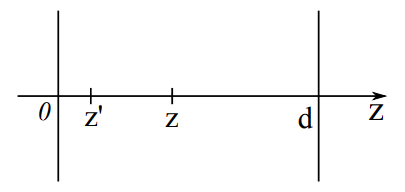
\includegraphics[scale=1]{pics/pic7.png}
\caption{Интерференция вторичных волн при генерации второй гармоники}
\end{figure}

Тогда для диполей, расположенных в некоторой плоскости $z^{'}$, колебания с удвоенной частотой $2\omega$ описываются, в соответствии с \eqref{x} функцией
\begin{equation}
X^{(2\omega)}(t, z^{'}) = A^2 \cos 2 \left[ \omega t + \varphi (z^{'}) \right]
\label{X}
\end{equation}
Где фаза $\varphi(z^{'})$ определяется фазовой скоростью первичной волны с частотой $\omega$
\begin{equation}
\varphi(z^{'}) = - k z^{'} = - \frac{\omega}{c} n(\omega) z^{'}
\end{equation}
$n(\omega)$ - показатель преломления среды. Тогда \eqref{X} запишется как
\begin{equation}
X^{(2\omega)} = A^2 \cos 2 \omega \left[t - \frac{n(\omega)}{c} z^{'} \right]
\end{equation}
Колеблющийся по данному закону диполь излучает вторичную волну частотой $2\omega$. Добавку фазы вторичной волны в какой-либо точке $z$ внутри нелинейной среды можно вычислить
\begin{equation}
\frac{2 \omega n(2\omega) (z^{'} - z)}{c}
\end{equation}
Тогда фаза колебаний в точке z равна
\begin{equation}
    \varphi(z) = 2 \omega \left[ t - \frac{n(\omega)}{c} z^{'} \right] - \frac{2 \omega n(2\omega)(z-z^{'})}{c}
\end{equation}
\begin{equation}
    \varphi(z)= 2 \omega \{ t - \frac{n(2\omega)}{c} z + \left[ n(2\omega) - n(\omega) \right] \frac{z^{'}}{c} \}
\label{phase}
\end{equation}
Полное поле на частоте $2\omega$ в точке z есть сумма вторичных, волн, испущенных диполями, расположенными между входной поверхностью среды и плоскостью $z$. Если показатели преломления $n(\omega)$ и $n(2\omega)$ одинаковые, то фаза \eqref{phase} не зависит от расположения излучающего диполя, соответственно все вторичные волны синфазны и амплитуда напряжённости $E^{2\omega}_0$ второй гармоники пропорциональна расстоянию z от входной плоскости.

Равенство показателей преломления называется условием пространственной синфазности и соответствует наибольшей интенсивности второй гармоники, генерируемой в данной нелинейной среде. 

В общем случае показатели преломления зависят от частоты, поэтому напряжённость волны удвоенной частоты можно найти как ($E^{(2\omega)} \sim d = eX$(поле диполя), ищем поле, как суперпозицию полей всех вторичных волн)
\begin{equation}
E^{2\omega} = gA^2 \int^z_0 \cos \{ 2\omega \left[ t - n(2\omega) \frac{z}{c} \right] + 2 \omega \Delta n \frac{z^{'}}{c} \} dz^{'}
\end{equation}
Где g - коэффициент пропорциональности. Тогда получается
\begin{equation}
E^{(2\omega)} = gA^2 z \frac{\sin \{k_0(\omega) \Delta n z \}}{k_0(\omega) \Delta n z} \cdot \cos \{2\omega\left( t - \frac{n(\omega) + n(2\omega)}{2c}z \right) \}
\label{sec_garm}
\end{equation}  
Как видно из \eqref{sec_garm}, амплитуда второй гармоники содержит интерфереционный множитель $sinc \left( k_0(\omega) \Delta n z \right)$, который отражает частичное или полное гашение вторичных волн, испущенных в различных точках среды.

На рисунке \ref{garm} приведена зависимость $| A^{(2\omega)} |$ от координаты z.

\begin{figure}[H]
\centering
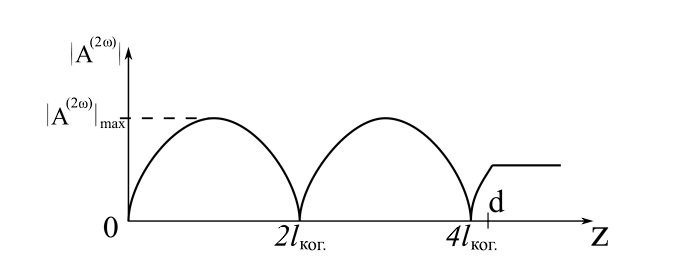
\includegraphics[scale=1]{pics/pic2.png}
\caption{Зависимость амплитуды второй гармоники $| A^{(2\omega)} |$ от расстояния z}
\label{garm}
\end{figure}

Здесь $l_\text{ког} = \frac{\lambda}{4 \Delta n}$ - длина когерентности. Из рисунка видно, что при распространении волны происходят последовательные процессы накопления интенсивности второй гармоники и затем обратная перекачка энергии из волны $E^{(2\omega)}$ в волну $E^{(\omega)}$.

Если выполняется условие синхронизма $\Delta n = 0$, то длина когерентности $l_\text{ког}$ становится бесконечно большой.

Можно добиться выполнения условия фазового синхронизма, если применить в качестве нелинейной среды анизотропные кристаллы. Так, в одноосном кристалле на рисунке \ref{refl} показатель преломления для волны, поляризованной перпендикулярно оптической оси z кристалла (обыкновенная волна), $n_o$ не зависит от направления распространения волны. Для волны же, поляризованной в плоскости оптической оси (необыкновенная волна), зависимость показателя преломления $n_e$ от направления распространения достаточно сильная.

Одноосные кристаллы, для которых $n_e - n_o > 0$, называются положительными, а
кристаллы, для которых $n_e - n_o < 0$, называются отрицательными.

Если двупреломление $|n_e - n_o|$ велико, возможно пересечение эллипсоида $n_e(2\omega)$ и сферы $n_o(\omega)$, и в направлении $\Theta_0$ с оптической осью для отрицательных кристаллов $n_o(\omega) = n_e(2\omega)$

\begin{figure}[H]
\centering
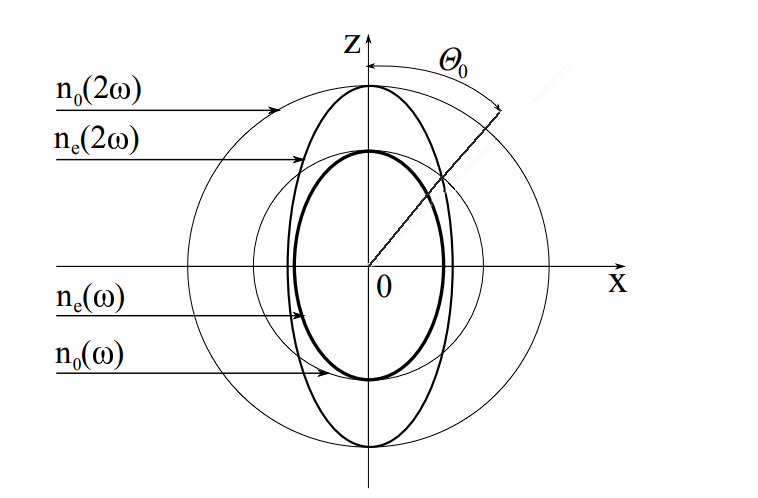
\includegraphics[scale=1]{pics/pic3.png}
\caption{Сечения поверхностей показателя преломления обыкновенной $n_o(\omega), n_o(2\omega)$, и необыкновенной $n_e(\omega), n_e(2\omega)$ волн}
\label{refl}
\end{figure}

Таким образом, выполняется условие синхронизма, если основная волна обыкновенная, а волна второй гармоники - необыкновенная.

Угол $\Theta_0$ называется углом синхронизма.
Также важно отметить, что в реальном эксперименте когерентная длина не обращается в бесконечность при выполнении условия синхронизма, что связано с расходимостью световых пучков, приводящей к отклонению части лучей от направления синхронизма. Влияние расхождения пучка будем определять специальным параметром - градиентом рассогласования $\frac{d \Delta}{d \Theta}$.

Для примера на рисунке 4 приведена зависимость интенсивности $I^{(2\omega)}(\Delta \Theta)$ второй гармоники в кристалле $LiNbO_3$ от угла между направлением распространения света $\Theta$ и направлением синхронизма $\Theta_0$.

\begin{figure}[H]
\centering
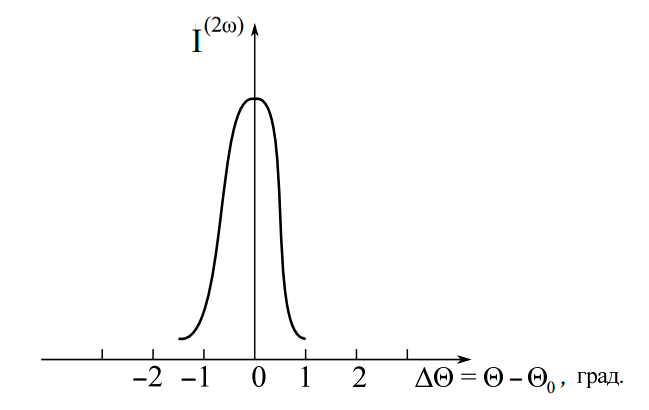
\includegraphics[scale=1]{pics/pic4.png}
\caption{Зависимость интенсивности второй гармоники $I^{(2\omega)}$ от угла $\Delta \Theta$ в кристалле $LiNbO_3$}
\label{int}
\end{figure}

Согласно соотношению \eqref{sec_garm}, амплитуда $A^{(2\omega)}$ волны с удвоенной частотой пропорциональная квадрату амплитуды падающей волны A, а это значит, что интенсивность излучения волны второй гармоники пропорциональна квадрату интенсивности исходного пучка. Однако это имеет место только в случае, если $I^{(2\omega)}$ составляет небольшую часть от $I^{(\omega)}$, так как энергия второй гармоники, как было показано выше, черпается из первичной волны.
\subsection*{Тензор нелинейной восприимчивости $\chi_{ikj}$. \\Нелинейный кристалл $LiNbO_3$}
Как было получено ранее, генерация второй гармоники определяется нелинейной поляризацией среды (cм. \eqref{pol})
\begin{equation}
P^{(2\omega)}_i = \sum_{j,k} \chi^{(2\omega)}_{ikj} E^{(\omega)}_j E^{(\omega)}_k
\label{2garm}
\end{equation}
где $\chi_{ijk}$ - тензор третьего ранга. Перестановка j и k не влияет на значение поляризации, получается имеет место симметрия
\begin{equation}
\chi^{(2\omega)}_{ijk} = \chi^{(2\omega)}_{ikj}
\end{equation}

Тогда данный тензор можно переписать в виде упрощённой матрицы(т.к. для каждому $i$ соответствуют 6, а не 9 различных значений, то матрица будет 3 на 6).

\begin{equation}
d_{im} = 1/2 \chi_{ikj}
\end{equation}
где
\begin{table}[H]
\begin{tabular}{c c c c c c c}
kj & 11 & 22 & 33 & 23, 32 & 31, 13 & 12, 21 \\
m & 1 & 2 & 3 & 4 & 5 & 6 \\
\end{tabular}
\end{table}

Тогда выражение \eqref{2garm} можно переписать в матричной форме
\begin{equation}
\begin{bmatrix}
P_x \\
P_y \\
P_z
\end{bmatrix}
= 
\begin{bmatrix}
d_{11} & d_{12} & d_{13} & d_{14} & d_{15} & d_{16} \\
d_{21} & d_{22} & d_{23} & d_{24} & d_{25} & d_{26} \\
d_{31} & d_{32} & d_{33} & d_{34} & d_{35} & d_{36}
\end{bmatrix}
\cdot
\begin{bmatrix}
E^2_x \\
E^2_y \\
E^2_x \\
2 E_y E_z \\
2 E_x E_z \\
2 E_x E_y
\end{bmatrix}
\label{mat}
\end{equation}
$d_{im}$ - тензор квадратичной нелинейной восприимчивости.

Число ненулевых членов в $d^{(2\omega)}_{im}$ зависит от группы точечной симметрии среды. Для применяемого кристалла ниобата лития $LiNbO_3$ (класс $3 - C_3$) данный тензор имеет вид
\begin{equation}
d_{im} =
\begin{bmatrix}
0 & 0 & 0 & 0 & d_{15} & -d_{22} \\
-d_{22} & d_{22} & 0 & d_{15} & 0 & 0 \\
d_{31} & d_{31} & d_{33} & 0 & 0 & 0
\end{bmatrix}
\end{equation}

Теперь, зная этот тензор для нашего случая, найдём чему равна интенсивность второй гармоники. Будет рассматривать такую первичную волну с частотой $\omega$, при которой выполняется условие синхронизма. Как уже было отмечено ранее, для этого падающая волна должна быть обыкновенной - её вектор напряженности $\vec{E^{(\omega)}}$ должен быть перпендикулярен оптической оси z. Пусть она распространяется в кристале под углом $\Theta$ к оптической оси z в плоскости, проходящей через оптическую ось и составляющей угол $\varphi$ с осью x (рисунок \ref{wave}).

\begin{figure}[H]
\centering
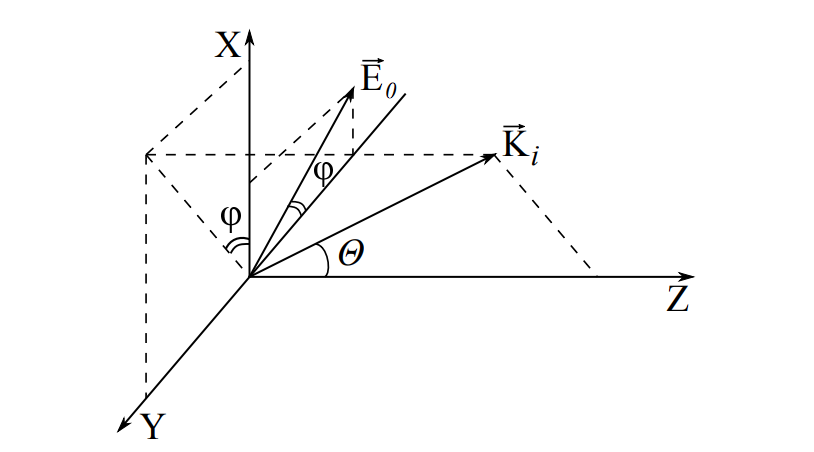
\includegraphics[scale=0.5]{pics/pic5.png}
\caption{Распространение обыкновенной волны относительно осей кристалла}
\label{wave}
\end{figure}
Как видно из геометрии, проекции вектора $\vec{E}$ на оси координат($\vec{E}$ перпендикулярен $\vec{k}$, а также оптической оси, значит он перпендикулярен всей плоскости kZ, а значит также перпендикулярен проекции вектора $\vec{k}$ на плоскость xy)

\[E_x = E_o \sin \varphi \]
\[E_y = - E_o \cos \varphi \]
\[E_z = 0\]

Тогда подставим в \eqref{mat}
\[P_x= 2d_{15}E_{x}E_{z} - 2d_{22}E_{x}E_{y} \]
\begin{equation}
P_y = -d_{22}E_{x}^2+d_{22}E_{y}^2+2d_{15}E_{y}E_{z}
\end{equation}
\[P_z = d_{31} (E^2_x +E^2_y) + d_{33}E_z^2\]



Тогда компонента нелинейной поляризации, дающая необыкновенную волну, равна(с учётом, что поле необыкновенной волны должно лежать на главной плоскости)
\begin{equation}
P_e = E_e^2(d_{31}\sin \theta + d_{22}\sin 3\varphi \cos \theta)
\end{equation}
Тогда в итоге, т.к. для колеблющихся диполей интенсивность задаётся формулой $I = \frac{2}{3c^3} |\ddot{P}|^2$, то интенсивность второй гармоники равна
\begin{equation}
I^{(2\omega)} = \frac{8 \omega^4}{3c^3} (d_{31}\sin \theta + d_{22} \sin 3\varphi \cos \theta)^2 \left( I^{(\omega)} \right)^2
\label{int}
\end{equation}
- и достаточно мала, так как условия измерения соответствующих компонент тензора далеки от синхронизма.

\section{Экспериментальная установка}
Оборудованием для изучения эффекта является лазер ЛТИ-501 (твердотельный лазер с длиной излучения $\lambda = 1064 \text{ нм}$ - ИК диапазон), нелинейный кристалл, система ориентации кристала, прибор ночного видения, система регистрации излучения второй гармоники.
Схема установки изображена на рис. \ref{fig:ust}
\begin{figure}[H]
	\centering
	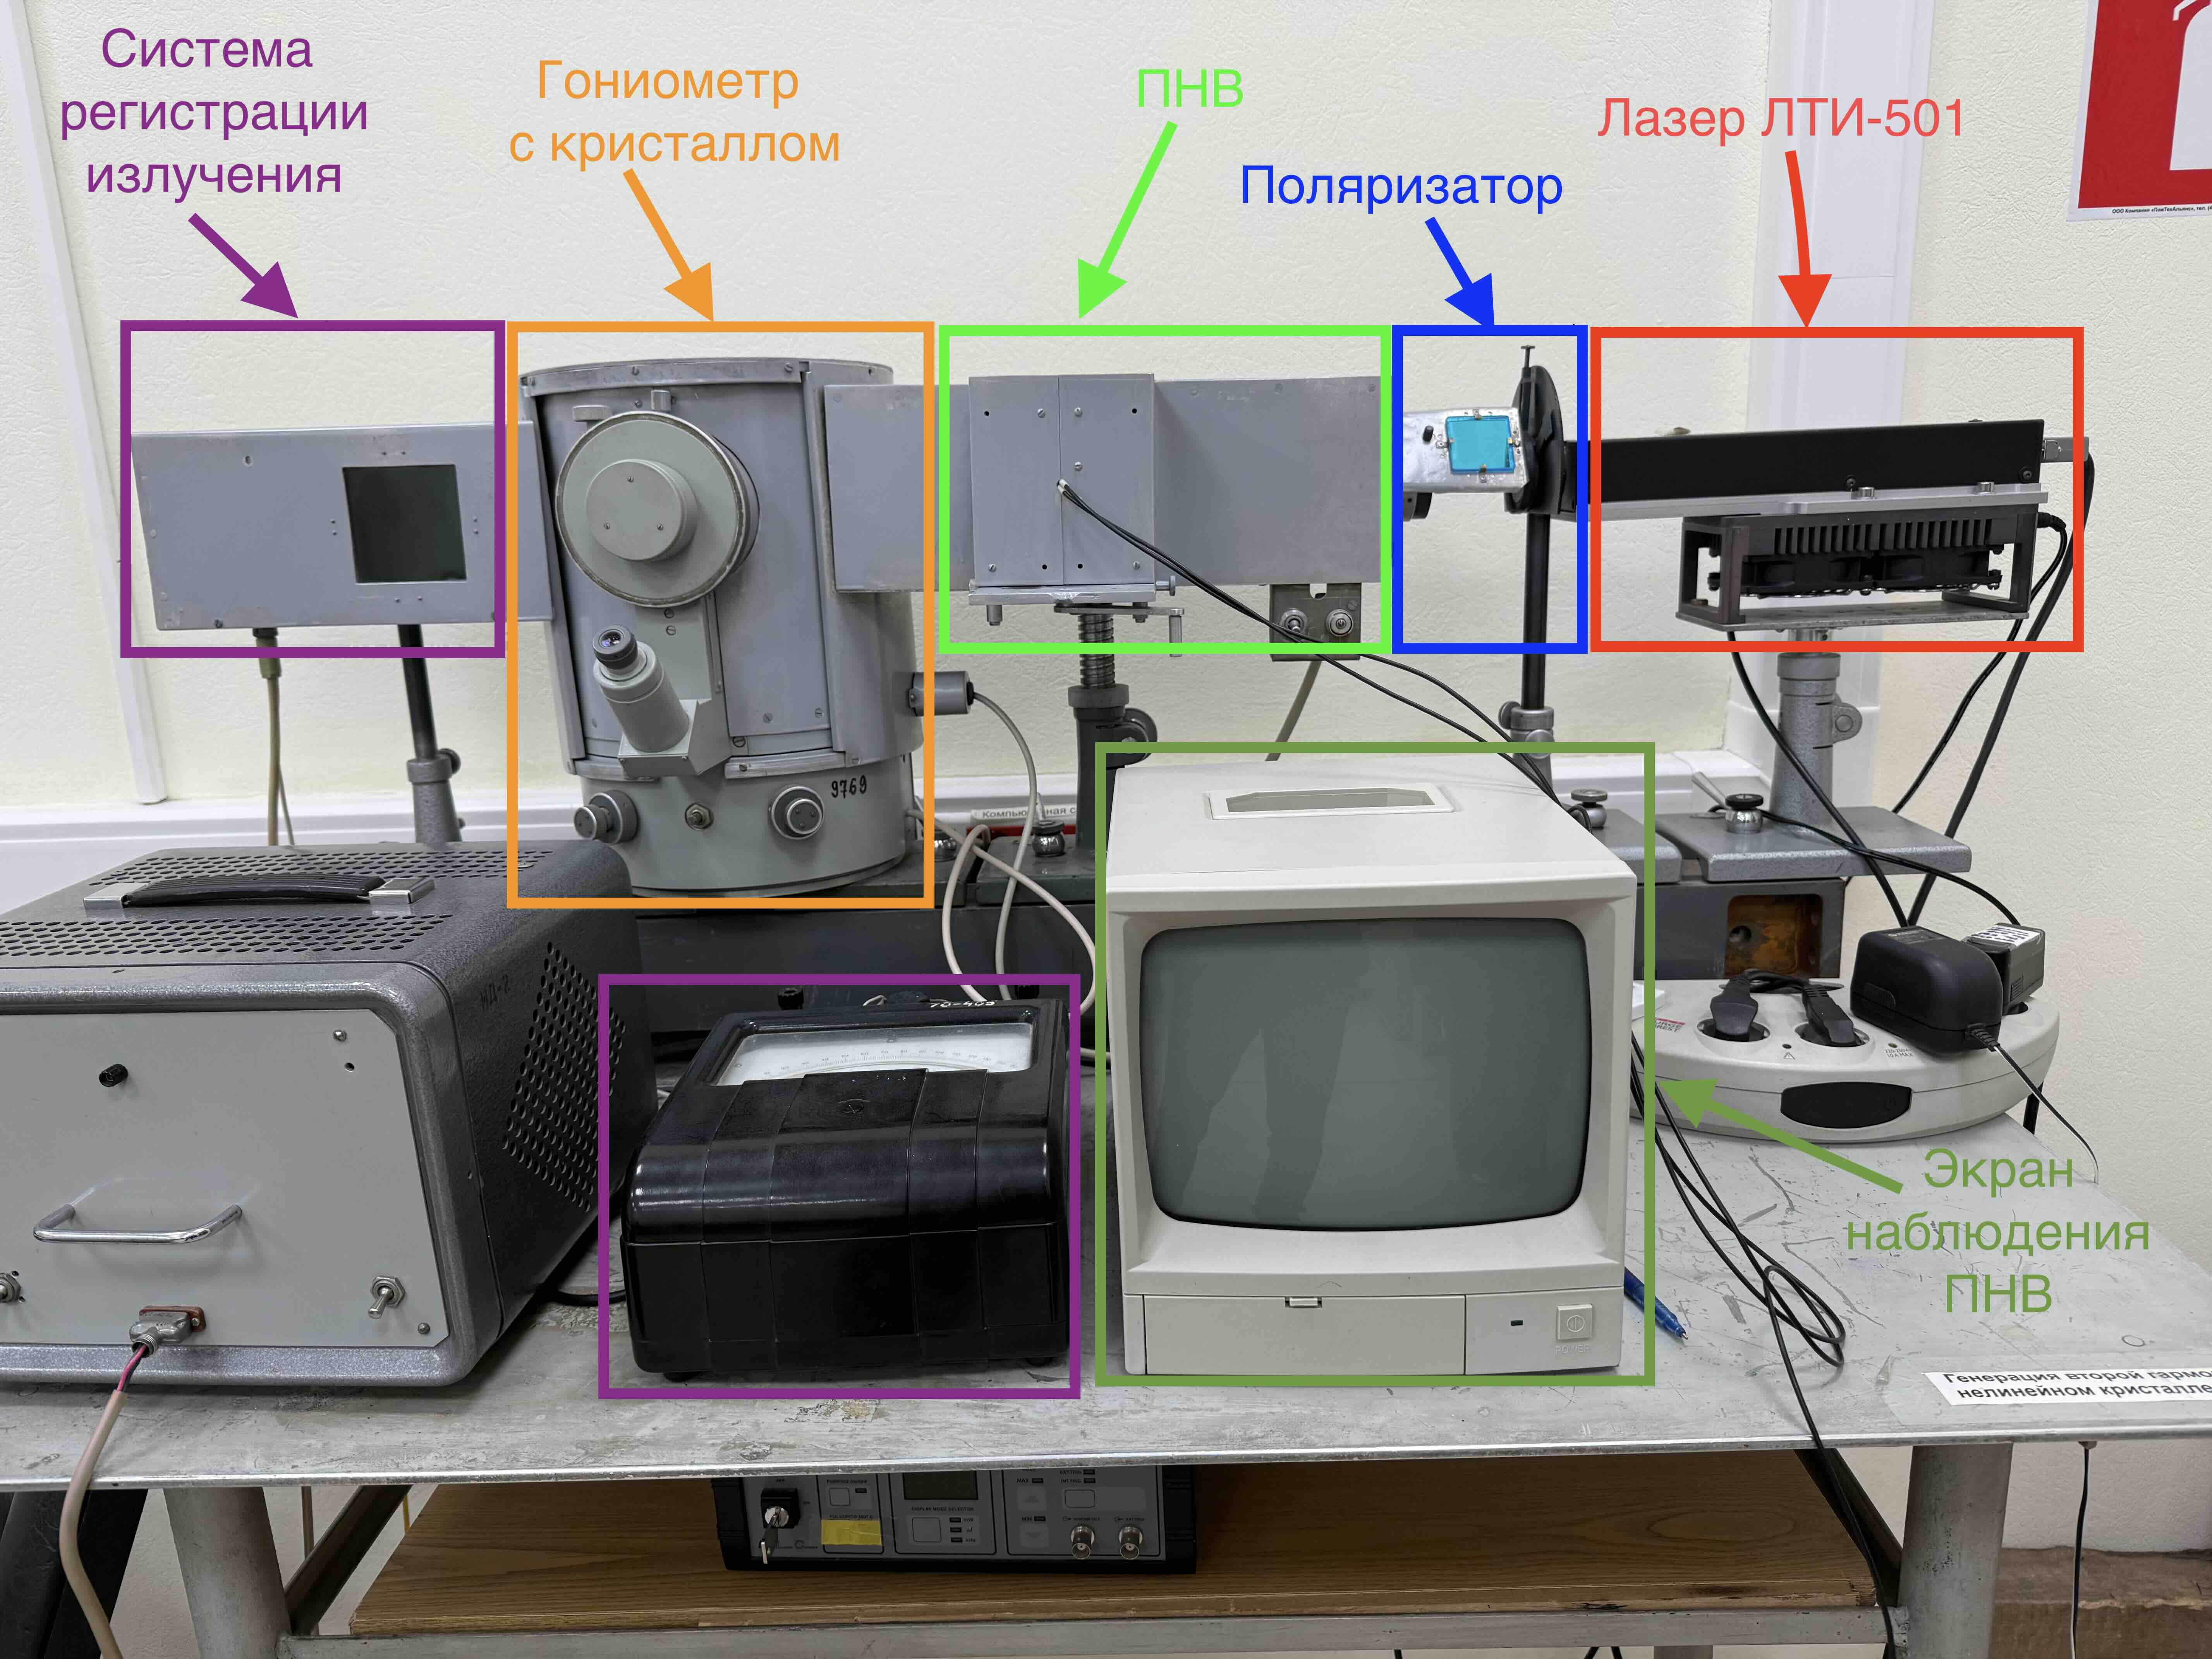
\includegraphics[height=0.5\textheight]{Ustanovka.jpg}
	\caption{Схема экспериментальной установки}
	\label{fig:ust}
\end{figure}
\section{Ход работы}
\subsection{Задание 1. Определение углов синхронизма в кристалле ниобата лития}
\subsubsection{Вычисление углов синхронизма}
Из теоретической справки, в частности, формулы \ref{sec_garm}, следует
\begin{equation}
    n_e(\theta) = n_0(1+((\frac{n_0}{n_e}) - 1) ^ 2 \sin ^2 \theta)^{-1/2}
\end{equation}
Используя значение $n_0 = 2,234$ при $\lambda = 1064$ нм и $n_0 = 2,323$ при $\lambda = 532$ нм, а также $n_e = 2,154$ при $\lambda = 1064$ нм и $n_e = 2,229$ при $\lambda = 532$ нм, вычислим значение углов синхронизма для исследуемого ниобата лития: $\theta_0 = 77 ^{\circ} + 180 ^{\circ} * k, k \in Z $ \\
Экспериметально определим углы попадания на диафрагму: $\varphi_1 = 155 ^{\circ}47' , \varphi_2 = 336^{\circ}09'$ \\
Затем, используя систему регистрации излучения второй гармоники, определим углы фазового синхронизма исследуемого образца: $\theta_{01}= 110 ^{\circ}8', \theta_{02} = 290^{\circ}10'$
\subsection{Задание 2. Исследование зависимости интенсивность второй гармоники от отклонения от угла синхронизма}
В первом задании были определены углы синхронизма для исследуемого кристалла.
Измерим интенсивность излучения второй гармоники для о-поляризованной (перпендикулярно оси Oz) и для е-поляризованной (параллельно оси Oz) волн.
Результаты отобразим в таблицах:
\begin{table}[H]
    \centering
    \label{tab:o_wave}
    \footnotesize
    \begin{tabular}{|c|c|c|c|c|c|c|}
        \hline
        $\theta$ (°,') & $I$ (мА) & $\theta$ (°,') & $I$ (мА) & $\theta$ (°,') & $I$ (мА) \\
        \hline
        109,52 & 58 & 109,54 & 55 & 109,56 & 68 \\
        109,58 & 77 & 110,00 & 99 & 110,02 & 121 \\
        110,04 & 138 & 110,06 & 147 & 110,08 & 153 \\
        110,10 & 147 & 110,12 & 140 & 110,13 & 123 \\
        110,14 & 103 & 110,16 & 79 & 110,18 & 63 \\
        110,20 & 57 & 110,22 & 45 & 110,24 & 48 \\
        \hline
    \end{tabular}
    \caption{Зависимость интенсивности от угла для О-поляризованной волны}
\end{table}

\vspace{0.2cm}

\begin{table}[H]
    \centering
    \label{tab:e_wave}
    \footnotesize
    \begin{tabular}{|c|c|c|c|c|c|c|}
        \hline
        $\theta$ (°,') & $I$ (мА) & $\theta$ (°,') & $I$ (мА) & $\theta$ (°,') & $I$ (мА) \\
        \hline
        289,56 & 51 & 289,58 & 50 & 290,00 & 46 \\
        290,02 & 65 & 290,04 & 94 & 290,06 & 113 \\
        290,08 & 126 & 290,10 & 131 & 290,12 & 128 \\
        290,14 & 112 & 290,16 & 91 & 290,18 & 62 \\
        290,20 & 53 & 290,22 & 45 & 290,24 & 47 \\
        290,26 & 48 & & & & \\
        \hline
    \end{tabular}
    \caption{Зависимость интенсивности от угла для e-поляризованной волны}
\end{table}

По этим данным были построены графики интенсивности от отклонения от угла синхронизма. Они представлены на рисунках ниже. 
\begin{figure}[H]
	\centering
	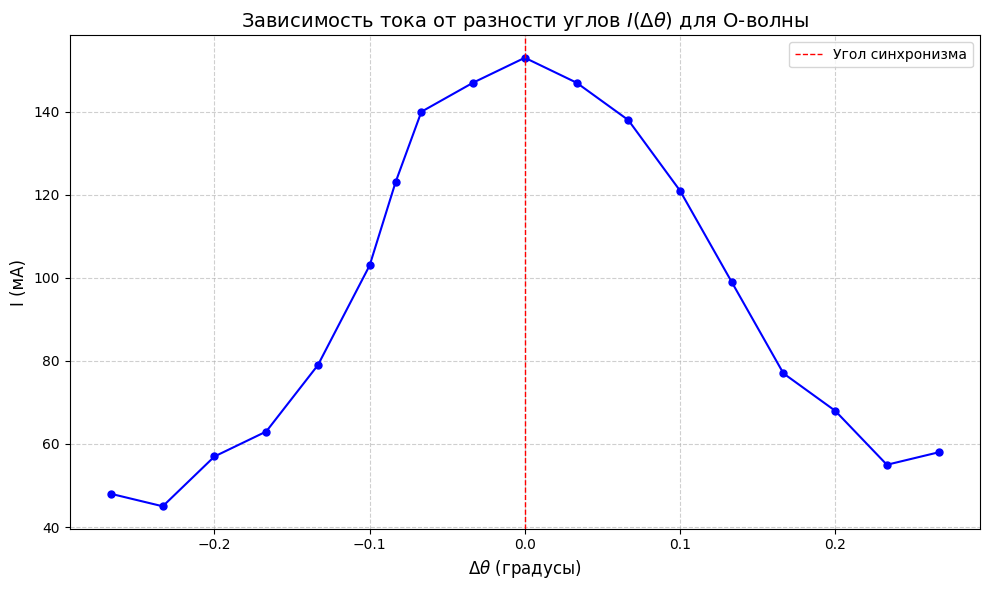
\includegraphics[height=0.4\textheight]{Unknown.png}
	\caption{График зависимости интенсивности от отклонения от угла синхронизма для О-поляризованной волны}
	\label{fig:gr1}
\end{figure}

\begin{figure}[H]
	\centering
	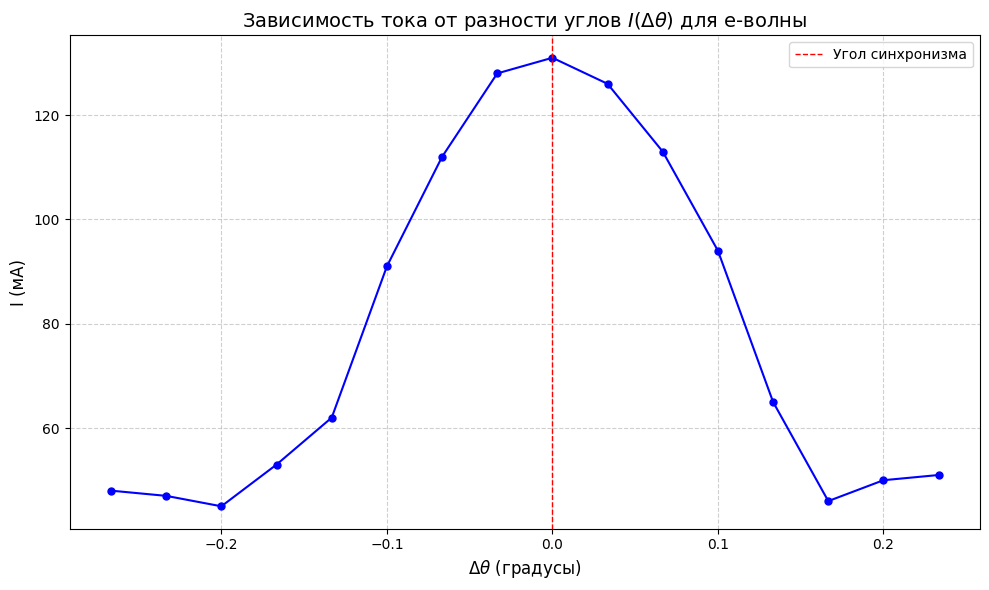
\includegraphics[height=0.4\textheight]{Unknown-2.png}
	\caption{График зависимости интенсивности от отклонения от угла синхронизма для е-поляризованной волны}
	\label{fig:gr2}
\end{figure}

\section{Вывод}
В ходе данной лабораторной работы было исследовано явление генерации второй гармоники в кристалле $LiNbO_3$, определены углы синхроизма образца, а также зависимость интенсивности второй гармоники от отклонения от угла синхронизма.
\end{document}
